%
%===================================================================================================
%
\documentclass[aspectratio=169]{beamer}
%
%===================================================================================================
%
% Theme and color scheme

\usetheme{Madrid}
\usecolortheme{default}

%
%===================================================================================================
%
% Define color

\definecolor{accent}{RGB}{180,40,40}
\definecolor{accentblue}{RGB}{51,102,170}
\definecolor{betacolor}{RGB}{34,139,34}
\definecolor{darkblue}{RGB}{0,51,102}
\definecolor{darkgreen}{RGB}{0,100,50}
\definecolor{dotcolor}{RGB}{200,80,0}
\definecolor{factorcolor}{RGB}{128,0,128}
\definecolor{lightgray}{RGB}{240,240,245}

\setbeamercolor{structure}{fg=darkblue}
\setbeamercolor{frametitle}{bg=darkblue, fg=white}
\setbeamercolor{title}{bg=darkblue, fg=white}
\setbeamercolor{block title}{bg=accentblue, fg=white}
\setbeamercolor{block body}{bg=lightgray}
\setbeamercolor{block title alerted}{bg=red!70!black, fg=white}
\setbeamercolor{block body alerted}{bg=red!5}
\setbeamercolor{block title example}{bg=darkgreen, fg=white}
\setbeamercolor{block body example}{bg=green!5}

%
%===================================================================================================
%
% Packages

\usepackage{amsmath, amssymb, amsfonts, bm, mathtools}
\usepackage{graphicx}
\usepackage{tikz}
\usetikzlibrary{arrows.meta, positioning, calc, decorations.pathreplacing, fit, shapes}
\usepackage{booktabs}
\usepackage{hyperref}
\usepackage{listings}
\usepackage{multicol}
\usepackage[most]{tcolorbox}

%
%===================================================================================================
%
% Math shortcuts

\newcommand{\E}{\mathbb{E}}
\newcommand{\R}{\mathbb{R}}
\DeclareMathOperator{\tr}{tr}
\DeclareMathOperator{\rank}{rank}

%
%===================================================================================================
%
% New Commands


%
%===================================================================================================
%
% Navigation

\setbeamertemplate{navigation symbols}{}
\setbeamertemplate{footline}{%
  \hfill\usebeamercolor[fg]{structure}%
  \textbf{Lecture 3A} ~--~ \insertframenumber/\inserttotalframenumber%
  \hspace*{6pt}\vspace{3pt}%
}

\setbeamertemplate{section in toc}{%
  \vspace{12pt}%  ← regola questo valore
  \inserttocsectionnumber.~\inserttocsection\par
}
%
%===================================================================================================
%
% Title page information

\author{Giovanni Della Lunga\\{\footnotesize giovanni.dellalunga@unibo.it}}
\title{Chapter 3\\Autoencoder Asset Pricing}
\subtitle{} % (optional)
\setbeamercovered{transparent} 
\institute{Advanced Topics in Artificial Intelligence} 
\date{Bologna - March, 2026} 

%
%===================================================================================================
%
\begin{document}
%
%===================================================================================================
%
\setbeamertemplate{subsection page}
{
  \begingroup
    %\begin{beamercolorbox}[sep=12pt,center]{section title}
      %\usebeamerfont{section title}
	  \centering 	     
      Section~\insertsectionnumber.\insertsubsectionnumber\par 
      \vspace{1cm}
    %\end{beamercolorbox}
    %\vspace*{-2pt}
    \begin{beamercolorbox}[sep=8pt,center,rounded=true]{title}
      \usebeamerfont{section title}
      \insertsubsection\par
    \end{beamercolorbox}
  \endgroup
}
%
%===================================================================================================
%
\AtBeginSection[]
{
  %\begin{frame}<beamer>
  %\footnotesize	
  %\frametitle{Outline}
  %\begin{multicols}{2}
  %\tableofcontents[currentsection]
  %\end{multicols}	  
  %\normalsize
  %\end{frame}
  \begin{frame}
  \vfill
  \centering
  \begin{beamercolorbox}[sep=8pt,center,shadow=true,rounded=true]{title}  	\usebeamerfont{title}\insertsectionhead\par%
  \end{beamercolorbox}
  \vfill
  \end{frame}
}
\AtBeginSubsection{\frame{\subsectionpage}}
%
%===================================================================================================
%
\begin{frame}
\titlepage
\end{frame}
%
%===================================================================================================
%
\begin{frame}{Contents}
\begin{multicols}{2}
\tableofcontents[
    sectionstyle=show,
    subsectionstyle=show
]
\end{multicols}
\end{frame}%__________________________________________________________________________
%
\section{The Conditional Autoencoder}
%__________________________________________________________________________
%
%__________________________________________________________________________
%
\subsection{The Big Picture}
%__________________________________________________________________________
%
\begin{frame}{Recap: Where We Left Off}

\textbf{From Lecture 2:}
\begin{itemize}
    \item \textbf{Part 1:} Static factor models $r_t = \beta f_t + u_t$; PCA extracts latent factors but $\beta$ is constant.
    \item \textbf{Part 2:} Linear autoencoder $=$ PCA (Proposition 1). Adding nonlinearity generalizes PCA.
    \item \textbf{Part 3:} IPCA makes $\beta$ depend on characteristics: $\beta(z_{i,t-1})' = z'_{i,t-1}\Gamma$ (linear). But linearity is restrictive -- theory predicts nonlinear relationships.
\end{itemize}

\vspace{0.5em}
\textbf{Today:} We enter the \textbf{core} of the paper -- the \emph{Conditional Autoencoder}, which:
\begin{enumerate}
    \item Models $\beta$ as a \textbf{nonlinear} function of characteristics (neural network)
    \item Estimates \textbf{latent} factors as portfolios (linear combinations of returns)
    \item Combines both via a \textbf{dot product} to predict returns
    \item Imposes the economic restriction of \textbf{no-arbitrage}
\end{enumerate}
\end{frame}
%
%..................................................................
%
\begin{frame}{The Model at the Highest Level (Eq.\ 9)}

The conditional autoencoder is, at the highest level, still a factor model:

\begin{block}{Equation (9) of the paper}
\vspace{-0.5em}
\[
\boxed{r_{i,t} = \beta'_{i,t-1}\, f_t + u_{i,t}}
\]
\end{block}

\vspace{0.3em}
\textbf{Same structure as IPCA -- but the key differences are:}

\vspace{0.3em}
\begin{center}
\renewcommand{\arraystretch}{1.4}
\begin{tabular}{lll}
\toprule
& \textbf{IPCA} & \textbf{Conditional Autoencoder} \\
\midrule
$\beta_{i,t-1}$ & $\Gamma' z_{i,t-1}$ (linear) & $\text{NN}(z_{i,t-1}; \theta)$ (\textbf{nonlinear}) \\
$f_t$ & Latent (from FOCs) & Linear combination of returns \\
Interactions & None (additive) & Learned by hidden layers \\
\bottomrule
\end{tabular}
\end{center}

\vspace{0.5em}
The model has \textbf{two sub-networks} that are trained \emph{jointly} end-to-end.
\end{frame}
%
%..................................................................
%
\begin{frame}{Bird's Eye View: Two Sub-Networks}

\begin{center}
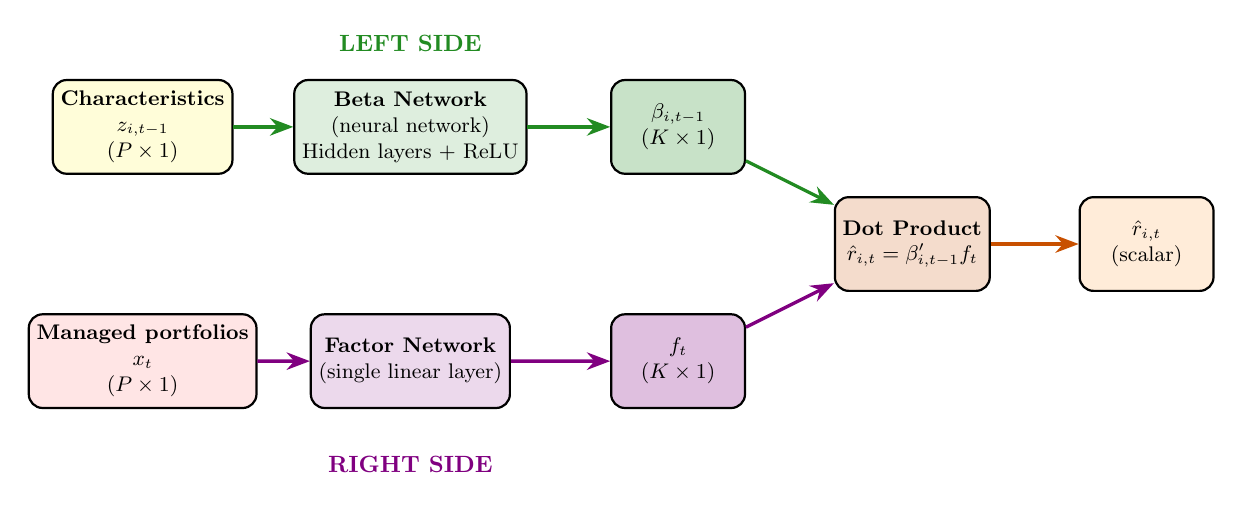
\begin{tikzpicture}[
    block/.style={draw, rounded corners=5pt, thick, minimum height=1.4cm, align=center, font=\small},
    >=Stealth, scale=0.85, every node/.style={scale=0.85}
]
  % Beta network
  \node[block, fill=yellow!15, minimum width=2.5cm] (Z) at (0, 0) {\textbf{Characteristics}\\$z_{i,t-1}$\\($P \times 1$)};
  
  \node[block, fill=betacolor!15, minimum width=2.5cm] (BNN) at (4, 0) {\textbf{Beta Network}\\(neural network)\\Hidden layers + ReLU};
  
  \node[block, fill=betacolor!25, minimum width=2.0cm] (Beta) at (8, 0) {$\beta_{i,t-1}$\\($K \times 1$)};
  
  \draw[->, very thick, betacolor] (Z) -- (BNN);
  \draw[->, very thick, betacolor] (BNN) -- (Beta);
  
  % Factor network
  \node[block, fill=red!10, minimum width=2.5cm] (X) at (0, -3.5) {\textbf{Managed portfolios}\\$x_t$\\($P \times 1$)};
  
  \node[block, fill=factorcolor!15, minimum width=2.5cm] (FNN) at (4, -3.5) {\textbf{Factor Network}\\(single linear layer)};
  
  \node[block, fill=factorcolor!25, minimum width=2.0cm] (F) at (8, -3.5) {$f_t$\\($K \times 1$)};
  
  \draw[->, very thick, factorcolor] (X) -- (FNN);
  \draw[->, very thick, factorcolor] (FNN) -- (F);
  
  % Dot product
  \node[block, fill=dotcolor!20, minimum width=2.0cm] (DOT) at (11.5, -1.75) {\textbf{Dot Product}\\$\hat{r}_{i,t} = \beta'_{i,t-1} f_t$};
  
  \draw[->, very thick, betacolor] (Beta) -- (DOT);
  \draw[->, very thick, factorcolor] (F) -- (DOT);
  
  % Output
  \node[block, fill=orange!15, minimum width=2.0cm] (OUT) at (15, -1.75) {$\hat{r}_{i,t}$\\(scalar)};
  
  \draw[->, very thick, dotcolor] (DOT) -- (OUT);
  
  % Labels
  \node[betacolor, font=\bfseries, above] at (4, 1.0) {LEFT SIDE};
  \node[factorcolor, font=\bfseries, below] at (4, -4.8) {RIGHT SIDE};
\end{tikzpicture}
\end{center}
\end{frame}
%
%..................................................................
%
\begin{frame}{What Each Network Does}

\begin{columns}[T]
\column{0.48\textwidth}
\begin{block}{Beta Network (left side)}
\textbf{Input:} $P$ firm characteristics $z_{i,t-1}$

\textbf{Output:} $K$ factor loadings $\beta_{i,t-1}$

\textbf{Architecture:} Deep neural network with ReLU activation and hidden layers

\textbf{Key feature:} Captures \emph{nonlinear} and \emph{interactive} effects of characteristics on risk exposures

\textbf{One network, applied to each stock $i$} (weights shared across stocks)
\end{block}

\column{0.48\textwidth}
\begin{block}{Factor Network (right side)}
\textbf{Input:} $P$ managed portfolios $x_t$ (or $N$ returns $r_t$)

\textbf{Output:} $K$ latent factor returns $f_t$

\textbf{Architecture:} Single \emph{linear} layer (no hidden layers, no activation)

\textbf{Key feature:} Factors remain \emph{portfolios} (linear combinations of returns) -- economically interpretable

\textbf{One network for the whole cross section}
\end{block}
\end{columns}
\end{frame}
%__________________________________________________________________________
%
\subsection{Beta network in detail}
%__________________________________________________________________________
%
\begin{frame}{The Beta Network: Mathematical Formulation}

The beta network transforms characteristics into factor loadings through $L_\beta$ hidden layers:

\begin{block}{Equations (10)--(12) of the paper}
\begin{align}
z^{(0)}_{i,t-1} &= z_{i,t-1} \tag{10}\\[6pt]
z^{(l)}_{i,t-1} &= g\!\left(b^{(l-1)} + W^{(l-1)} z^{(l-1)}_{i,t-1}\right), \quad l = 1, \ldots, L_\beta \tag{11}\\[6pt]
\beta_{i,t-1} &= b^{(L_\beta)} + W^{(L_\beta)} z^{(L_\beta)}_{i,t-1} \tag{12}
\end{align}
\end{block}

\vspace{0.3em}
\textbf{Eq.\ (10):} Initialize with raw characteristics (input layer).\\
\textbf{Eq.\ (11):} Apply nonlinear transformation (ReLU) at each hidden layer.\\
\textbf{Eq.\ (12):} Output layer is \textbf{linear} (no activation) -- produces $K$ beta values.
\end{frame}
%
%..................................................................
%
\begin{frame}{Equation (10): Initialization}

\[
z^{(0)}_{i,t-1} = z_{i,t-1} \in \R^{P \times 1}
\]

\vspace{0.5em}
\textbf{What is $z_{i,t-1}$?}
\begin{itemize}
    \item A vector of $P$ observable characteristics (94 in the original paper) for stock $i$ at time $t-1$
    \item Includes: momentum, size, value, volatility, liquidity, profitability, investment, \ldots
    \item All characteristics are \textbf{rank-normalized} into $(-1, 1)$ each month
    \item Missing values replaced by the cross-sectional median
    \item Characteristics are \textbf{lagged}: we use $z_{i,t-1}$ to predict returns at time $t$
\end{itemize}

\vspace{0.5em}
\textbf{Why normalize?}
\begin{itemize}
    \item Raw characteristics have very different scales (market cap in billions vs.\ beta $\approx 1$)
    \item Rank normalization ensures all inputs are comparable and bounded
    \item Prevents outliers from dominating the network
    \item Makes optimization more stable
\end{itemize}
\end{frame}
%
%..................................................................
%
\begin{frame}{Equation (11): Hidden Layer Propagation}

For each hidden layer $l = 1, \ldots, L_\beta$:
\[
z^{(l)}_{i,t-1} = g\!\left(b^{(l-1)} + W^{(l-1)} z^{(l-1)}_{i,t-1}\right)
\]

\vspace{0.3em}
\textbf{Components:}
\begin{itemize}
    \item $W^{(l-1)} \in \R^{K^{(l)} \times K^{(l-1)}}$: weight matrix connecting layer $l-1$ to layer $l$
    \item $b^{(l-1)} \in \R^{K^{(l)}}$: bias vector for layer $l$
    \item $g(\cdot) = \max(\cdot, 0)$: ReLU activation (applied element-wise)
    \item $K^{(l)}$: number of neurons in layer $l$
\end{itemize}

\vspace{0.5em}
\textbf{What happens at each layer:}
\begin{enumerate}
    \item \textbf{Linear transformation:} $W^{(l-1)} z^{(l-1)}_{i,t-1} + b^{(l-1)}$ -- mixes and recombines features
    \item \textbf{Nonlinear activation:} ReLU sets negative values to zero -- creates \emph{sparsity} and \emph{piecewise linearity}
\end{enumerate}

\vspace{0.3em}
\textbf{Crucial:} The \textbf{same weights} $W^{(l)}, b^{(l)}$ are used for \emph{every} stock $i$. The only thing that changes across stocks is the input $z_{i,t-1}$.
\end{frame}
%
%..................................................................
%
\begin{frame}{Where Nonlinearity and Interactions Come From}

\textbf{Example:} Two characteristics $z_1$ (momentum) and $z_2$ (size).

\vspace{0.3em}
After one hidden layer with 2 neurons:
\[
h_1 = \max(0,\; w_{11}z_1 + w_{12}z_2 + b_1), \qquad h_2 = \max(0,\; w_{21}z_1 + w_{22}z_2 + b_2)
\]

Output: $\beta_k = v_1 h_1 + v_2 h_2 + b_k^{\text{out}}$

\vspace{0.5em}
\textbf{This captures:}
\begin{itemize}
    \item \textbf{Nonlinear effects:} $\beta$ changes slope at different levels of $z_1$ (due to ReLU kink)
    \item \textbf{Interactions:} $h_1$ mixes $z_1$ and $z_2$ together, so $\beta$ depends on their \emph{combination}
    \item \textbf{Threshold effects:} If $w_{11}z_1 + w_{12}z_2 + b_1 < 0$, neuron $h_1$ is off -- $\beta$ depends only on $h_2$
\end{itemize}

\vspace{0.5em}
\begin{exampleblock}{Compare with IPCA}
IPCA: $\beta_k = \gamma_{k1} z_1 + \gamma_{k2} z_2$ (purely additive, no interactions, no thresholds).
The neural network is a \textbf{strict generalization}.
\end{exampleblock}
\end{frame}
%
%..................................................................
%
\begin{frame}{Equation (12): The Output Layer}

\[
\beta_{i,t-1} = b^{(L_\beta)} + W^{(L_\beta)} z^{(L_\beta)}_{i,t-1} \in \R^{K \times 1}
\]

\vspace{0.5em}
\textbf{The output layer is linear} (no ReLU). Why?
\begin{itemize}
    \item Factor loadings $\beta_{i,k}$ can be positive or negative
    \item ReLU would clip negative betas to zero -- destroying important information
    \item We want betas to be \emph{unconstrained} real numbers
\end{itemize}

\vspace{0.5em}
\textbf{Output dimensionality:}
\begin{itemize}
    \item $W^{(L_\beta)} \in \R^{K \times K^{(L_\beta)}}$: maps from last hidden layer to $K$ outputs
    \item Each output neuron represents one \textbf{factor loading} $\beta_{i,k}$ for $k = 1, \ldots, K$
    \item So the full output is $\beta_{i,t-1} = (\beta_{i,1,t-1}, \ldots, \beta_{i,K,t-1})'$
\end{itemize}

\vspace{0.5em}
\textbf{For each stock $i$ at each time $t$:} the network produces a \emph{personalized} vector of $K$ risk exposures, determined by that stock's current characteristics.
\end{frame}
%
%..................................................................
%
\begin{frame}{Weight Sharing Across Stocks}

\textbf{Critical design feature:} The beta network has \textbf{shared weights}.

\vspace{0.5em}
The same parameters $\{W^{(l)}, b^{(l)}\}_{l=0}^{L_\beta}$ are used for \emph{all} stocks $i = 1, \ldots, N$.

\vspace{0.5em}
\textbf{What changes across stocks:} Only the input $z_{i,t-1}$.

\vspace{0.5em}
\textbf{Why this matters:}
\begin{itemize}
    \item Without weight sharing: would need $\sim 30{,}000 \times (\text{parameters per stock})$ -- infeasible
    \item With weight sharing: the network learns a \emph{universal mapping} from characteristics to betas
    \item A new stock (IPO) gets immediate beta estimates -- just feed its characteristics through the trained network
    \item Stocks with similar characteristics get similar betas -- a form of \emph{regularization}
\end{itemize}

\vspace{0.5em}
\textbf{Analogy:} Think of the beta network as a ``beta calculator'' -- you input a stock's characteristics, and it outputs that stock's risk profile. The calculator is the same for everyone; the results differ because the inputs differ.
\end{frame}
%__________________________________________________________________________
%
\subsection{Factor network in detail}
%__________________________________________________________________________
%
\begin{frame}{The Factor Network: Overview}

\textbf{The right side of Figure 2} estimates the latent factors $f_t$.

\vspace{0.5em}
Ideally, we would use the full cross section of returns $r_t \in \R^N$:
\begin{align}
r^{(0)}_t &= r_t \tag{13}\\
r^{(l)}_t &= g\!\left(\tilde{b}^{(l-1)} + \tilde{W}^{(l-1)} r^{(l-1)}_t\right), \quad l = 1, \ldots, L_f \tag{14}\\
f_t &= \tilde{b}^{(L_f)} + \tilde{W}^{(L_f)} r^{(L_f)}_t \tag{15}
\end{align}

\vspace{0.5em}
\textbf{But there's a big problem\ldots}
\end{frame}
%
%..................................................................
%
\begin{frame}{The Dimensionality Problem}

\textbf{Why we can't use $r_t$ directly:}

\vspace{0.5em}
\textbf{Problem 1: Too many parameters.}
\begin{itemize}
    \item With $N \approx 30{,}000$ stocks: the first layer would need $K \times 30{,}000$ weight parameters
    \item With $T = 720$ months: massively more parameters than observations
    \item Guaranteed to overfit catastrophically
\end{itemize}

\vspace{0.5em}
\textbf{Problem 2: Unbalanced panel.}
\begin{itemize}
    \item On average $\sim$6,200 stocks per month, but different stocks each month
    \item Total universe: $\sim$30,000 stocks (enter/exit due to IPOs, delistings, mergers)
    \item Most stock-level weights would be estimated from very few time-series observations
\end{itemize}

\vspace{0.5em}
\begin{alertblock}{We need a way to reduce dimensionality \emph{before} entering the network.}
\end{alertblock}
\end{frame}
%
%..................................................................
%
\begin{frame}{The Solution: Managed Portfolios (Eq.\ 16)}

\textbf{Key insight:} Replace the $N$-dimensional return vector with $P$-dimensional managed portfolios.

\begin{block}{Equation (16) of the paper}
\vspace{-0.5em}
\[
\boxed{x_t = (Z'_{t-1} Z_{t-1})^{-1} Z'_{t-1}\, r_t}
\]
\end{block}

\vspace{0.3em}
\textbf{Dimensions:}
\begin{itemize}
    \item $Z_{t-1} \in \R^{N_t \times P}$: matrix of characteristics for all $N_t$ stocks at time $t-1$
    \item $r_t \in \R^{N_t}$: returns of all $N_t$ stocks at time $t$
    \item $x_t \in \R^{P}$: vector of $P = 94$ managed portfolio returns (plus one market portfolio)
\end{itemize}

\vspace{0.3em}
This is a \textbf{cross-sectional regression} of returns on characteristics at each time $t$:
\[
x_t = \arg\min_{x} \| r_t - Z_{t-1}\, x \|^2
\]

The $j$-th element of $x_t$ is the return on a long-short portfolio sorted by characteristic $j$.
\end{frame}
%
%..................................................................
%
\begin{frame}{Three Benefits of Using Managed Portfolios}

\textbf{Benefit 1: Massive dimensionality reduction.}
\begin{itemize}
    \item From $N \approx 30{,}000$ individual returns to $P = 95$ portfolio returns
    \item Eliminates tens of thousands of parameters from the factor network
\end{itemize}

\vspace{0.3em}
\textbf{Benefit 2: Handles panel incompleteness.}
\begin{itemize}
    \item Portfolios are formed from whichever stocks are available at each point in time
    \item No need for a balanced panel -- new stocks and delistings are handled automatically
\end{itemize}

\vspace{0.3em}
\textbf{Benefit 3: Connection to the finance literature.}
\begin{itemize}
    \item Characteristic-managed portfolios are well-studied (KPS, Feng et al., Kozak et al.)
    \item KPS and Giglio \& Xiu show that conditional linear models for individual stocks can be recast as static factor analysis on managed portfolios
    \item Provides a natural bridge between individual stock models and portfolio-level analysis
\end{itemize}
\end{frame}
%
%..................................................................
%
\begin{frame}{Managed Portfolios as a Pre-Processing Layer}

\textbf{Conceptual view:} $x_t$ adds a new initial layer to the factor network.

\vspace{0.5em}
\begin{center}
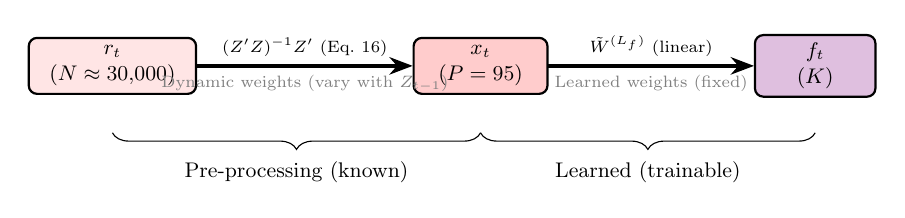
\begin{tikzpicture}[
    layer/.style={draw, rounded corners=3pt, thick, minimum height=0.8cm, align=center, font=\small},
    >=Stealth, scale=0.85, every node/.style={scale=0.85}
]
  \node[layer, fill=red!10, minimum width=2.5cm] (R) at (0, 0) {$r_t$\\($N \approx 30{,}000$)};
  
  \node[layer, fill=red!20, minimum width=2.0cm] (X) at (5.5, 0) {$x_t$\\($P = 95$)};
  
  \node[layer, fill=factorcolor!25, minimum width=1.8cm] (F) at (10.5, 0) {$f_t$\\($K$)};
  
  \draw[->, very thick] (R) -- node[above, font=\scriptsize] {$(Z'Z)^{-1}Z'$ (Eq.\ 16)} node[below, font=\scriptsize, gray] {Dynamic weights (vary with $Z_{t-1}$)} (X);
  \draw[->, very thick] (X) -- node[above, font=\scriptsize] {$\tilde{W}^{(L_f)}$ (linear)} node[below, font=\scriptsize, gray] {Learned weights (fixed)} (F);
  
  \draw[decorate, decoration={brace, amplitude=6pt, mirror}] (0, -1.0) -- (5.5, -1.0);
  \node[below, font=\small] at (2.75, -1.3) {Pre-processing (known)};
  
  \draw[decorate, decoration={brace, amplitude=6pt, mirror}] (5.5, -1.0) -- (10.5, -1.0);
  \node[below, font=\small] at (8.0, -1.3) {Learned (trainable)};
\end{tikzpicture}
\end{center}

\vspace{0.5em}
The pre-processing step dynamically reweights stocks based on their characteristics -- it's a data-driven dimensionality reduction that varies over time.
\end{frame}
%
%..................................................................
%
\begin{frame}{The Factor Network: Final Specification}

With managed portfolios as input, the factor network becomes very simple:

\vspace{0.5em}
\textbf{Single linear layer} ($L_f = 1$, no hidden layers, no activation):
\[
f_t = \tilde{b}^{(L_f)} + \tilde{W}^{(L_f)}\, x_t
\]

\textbf{Dimensions:} $\tilde{W}^{(L_f)} \in \R^{K \times P}$, $\tilde{b}^{(L_f)} \in \R^K$.

\vspace{0.5em}
\textbf{Why keep the factor network linear?}

\begin{exampleblock}{Economic interpretability}
\begin{itemize}
    \item $f_t = \tilde{W}\, x_t + \tilde{b}$: each factor is a \textbf{linear combination of portfolio returns}
    \item Linear combinations of returns are themselves \textbf{portfolios}
    \item So factors are tradeable -- they have direct economic meaning
    \item A nonlinear factor network would produce factors that are \emph{not} portfolios, losing interpretability
\end{itemize}
\end{exampleblock}
\end{frame}
%__________________________________________________________________________
%
\subsection{Dot Product and Full Model}
%__________________________________________________________________________
%
\begin{frame}{The Dot Product: Combining Both Networks}

The final prediction for stock $i$ at time $t$:

\begin{block}{Output}
\vspace{-0.5em}
\[
\boxed{\hat{r}_{i,t} = \beta'_{i,t-1}\, f_t = \sum_{k=1}^{K} \beta_{i,k,t-1} \cdot f_{k,t}}
\]
\end{block}

\vspace{0.3em}
This is a \textbf{dot product} (inner product) between:
\begin{itemize}
    \item $\beta_{i,t-1} \in \R^K$: from the beta network (stock-specific, time-varying)
    \item $f_t \in \R^K$: from the factor network (common to all stocks, time-varying)
\end{itemize}

\vspace{0.5em}
\textbf{For the full cross section at time $t$:}
\[
\hat{r}_t = B_{t-1}\, f_t \in \R^N
\]
where $B_{t-1} = (\beta_{1,t-1}, \ldots, \beta_{N,t-1})' \in \R^{N \times K}$ is the matrix of all betas.

\vspace{0.3em}
This is exactly a factor model: $\hat{r}_t = \beta_t f_t$, but with \textbf{time-varying, nonlinear} betas.
\end{frame}
%
%..................................................................
%
\begin{frame}{The Dot Product as a Bilinear Operation}

\begin{center}
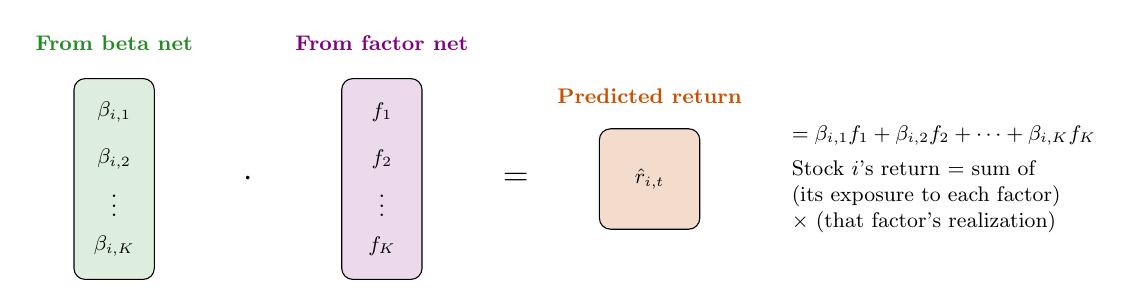
\begin{tikzpicture}[scale=0.85, every node/.style={scale=0.85}]
  % Beta vector
  \node[draw, rounded corners, fill=betacolor!15, minimum width=1.2cm, minimum height=3cm] (BETA) at (0, 0) {};
  \node[font=\small] at (0, 1.0) {$\beta_{i,1}$};
  \node[font=\small] at (0, 0.3) {$\beta_{i,2}$};
  \node at (0, -0.3) {$\vdots$};
  \node[font=\small] at (0, -1.0) {$\beta_{i,K}$};
  \node[above, font=\bfseries\small, betacolor] at (0, 1.8) {From beta net};
  
  % Times symbol
  \node[font=\Large] at (2, 0) {$\cdot$};
  
  % Factor vector
  \node[draw, rounded corners, fill=factorcolor!15, minimum width=1.2cm, minimum height=3cm] (FACT) at (4, 0) {};
  \node[font=\small] at (4, 1.0) {$f_1$};
  \node[font=\small] at (4, 0.3) {$f_2$};
  \node at (4, -0.3) {$\vdots$};
  \node[font=\small] at (4, -1.0) {$f_K$};
  \node[above, font=\bfseries\small, factorcolor] at (4, 1.8) {From factor net};
  
  % Equals
  \node[font=\Large] at (6, 0) {$=$};
  
  % Output
  \node[draw, rounded corners, fill=dotcolor!20, minimum width=1.5cm, minimum height=1.5cm] (OUT) at (8, 0) {};
  \node[font=\small] at (8, 0) {$\hat{r}_{i,t}$};
  \node[above, font=\bfseries\small, dotcolor] at (8, 1.0) {Predicted return};
  
  % Expansion
  \node[right, font=\small, align=left] at (10, 0) {$= \beta_{i,1} f_1 + \beta_{i,2} f_2 + \cdots + \beta_{i,K} f_K$\\[4pt]
  Stock $i$'s return $=$ sum of\\
  (its exposure to each factor)\\
  $\times$ (that factor's realization)};
\end{tikzpicture}
\end{center}

\vspace{0.5em}
\textbf{Key:} The dot product enforces the \textbf{factor model structure}. Without it, the network would be a generic prediction model (like GKX, 2019) with no economic structure.
\end{frame}
%
%..................................................................
%
\begin{frame}{Complete Forward Pass: Step by Step}

\textbf{For stock $i$ at time $t$, the conditional autoencoder computes:}

\vspace{0.5em}
\begin{enumerate}
    \item \textbf{Read characteristics:} $z_{i,t-1} \in \R^{P}$ (lagged, rank-normalized)
    
    \vspace{0.2em}
    \item \textbf{Beta network:} $z_{i,t-1} \xrightarrow{W^{(0)}, \text{ReLU}} h_1 \xrightarrow{W^{(1)}, \text{ReLU}} h_2 \xrightarrow{W^{(2)}, \text{linear}} \beta_{i,t-1} \in \R^K$
    
    
    \vspace{0.2em}
    \item \textbf{Compute managed portfolios:} $x_t = (Z'_{t-1}Z_{t-1})^{-1}Z'_{t-1}\,r_t \in \R^{95}$
    
    \quad (pre-processing, done once for all stocks at time $t$)
    
    \vspace{0.2em}
    \item \textbf{Factor network:} $x_t \xrightarrow{\tilde{W}, \text{linear}} f_t \in \R^K$
    
    \vspace{0.2em}
    \item \textbf{Dot product:} $\hat{r}_{i,t} = \beta'_{i,t-1}\, f_t \in \R$
\end{enumerate}

\vspace{0.5em}
\textbf{Repeat for all $N_t$ stocks at time $t$, then for all $T$ months.}
\end{frame}
%
%..................................................................
%
\begin{frame}{The Role of Each Component: Summary Table}

\begin{center}
\renewcommand{\arraystretch}{1.5}
\begin{tabular}{p{2.8cm} p{3.5cm} p{3.5cm} p{3.0cm}}
\toprule
\textbf{Component} & \textbf{Input} & \textbf{Output} & \textbf{Key property} \\
\midrule
\textcolor{betacolor}{\textbf{Beta network}} & $z_{i,t-1} \in \R^{94}$ (characteristics) & $\beta_{i,t-1} \in \R^K$ (loadings) & Nonlinear, shared weights \\
\textcolor{factorcolor}{\textbf{Factor network}} & $x_t \in \R^{95}$ (managed portfolios) & $f_t \in \R^K$ (factors) & Linear, factors $=$ portfolios \\
\textcolor{dotcolor}{\textbf{Dot product}} & $\beta_{i,t-1}$, $f_t$ & $\hat{r}_{i,t}$ (scalar) & Enforces factor structure \\
\textbf{Managed port.} & $r_t, Z_{t-1}$ & $x_t$ & Pre-processing, not learned \\
\bottomrule
\end{tabular}
\end{center}
\end{frame}
%
%..................................................................
%
\begin{frame}{Why This Architecture?}

The design of the conditional autoencoder reflects a careful balance of \textbf{economic structure} and \textbf{statistical flexibility}:

\vspace{0.5em}
\begin{itemize}
    \item \textbf{Factor model structure} ($r = \beta' f + u$): preserved via the dot product. This is not a black-box predictor -- it's an asset pricing model.
    
    \vspace{0.3em}
    \item \textbf{Nonlinear betas:} The neural network allows flexible, data-driven risk exposures that capture interactions and thresholds.
    
    \vspace{0.3em}
    \item \textbf{Linear factors:} Keeping factors as portfolios maintains economic interpretability and connects to the finance literature.
    
    \vspace{0.3em}
    \item \textbf{Managed portfolios:} Solve the dimensionality and unbalanced panel problems elegantly.
    
    \vspace{0.3em}
    \item \textbf{Weight sharing:} Makes the model feasible for $\sim$30,000 stocks and provides implicit regularization.
    
    \vspace{0.3em}
    \item \textbf{No intercept:} Imposes the no-arbitrage restriction (more in Part B).
\end{itemize}
\end{frame}
%
%..................................................................
%
\begin{frame}{What Makes This a ``Conditional'' Autoencoder?}

\textbf{Standard autoencoder} (Lecture 2):
\begin{itemize}
    \item Input: returns $r_t$
    \item Hidden: factors (bottleneck)
    \item Output: reconstructed returns $\hat{r}_t$
    \item \textbf{Unsupervised:} uses only returns
\end{itemize}

\vspace{0.5em}
\textbf{Conditional autoencoder} (this paper):
\begin{itemize}
    \item \textbf{Conditions} the loadings on external information $z_{i,t-1}$
    \item Returns enter only through managed portfolios on the factor side
    \item Characteristics enter only on the beta side
    \item \textbf{Semi-supervised:} uses returns \emph{and} characteristics
\end{itemize}

\vspace{0.5em}
The conditioning is what allows betas to be \textbf{time-varying} and \textbf{stock-specific}: two stocks with different characteristics at the same time will have different betas, and the same stock at different times (with changed characteristics) will have different betas.
\end{frame}
%__________________________________________________________________________
%
\subsection{Conclusions and Summary}
%__________________________________________________________________________
%
\begin{frame}{Part A -- Summary}

\begin{enumerate}
    \item The conditional autoencoder maintains the factor model structure $r_{i,t} = \beta'_{i,t-1} f_t + u_{i,t}$, but with two neural sub-networks.
    
    \vspace{0.2em}
    \item The \textcolor{betacolor}{\textbf{beta network}} (Eqs.\ 10--12) maps 94 characteristics to $K$ loadings through hidden layers with ReLU activation. Architectures: CA0 (linear), CA1 (32), CA2 (32-16), CA3 (32-16-8).
    
    \vspace{0.2em}
    \item The \textcolor{factorcolor}{\textbf{factor network}} (Eqs.\ 13--16) uses managed portfolios $x_t$ as input and a single linear layer, keeping factors interpretable as portfolios.
    
    \vspace{0.2em}
    \item Managed portfolios (Eq.\ 16) solve the dimensionality and unbalanced panel problems by reducing $N \approx 30{,}000$ returns to $P = 95$ portfolio returns.
    
    \vspace{0.2em}
    \item The \textcolor{dotcolor}{\textbf{dot product}} $\hat{r}_{i,t} = \beta'_{i,t-1} f_t$ combines both networks and enforces the factor model structure.
    
    \vspace{0.2em}
    \item Weight sharing across stocks keeps the model tractable ($\sim$4,000 parameters).
\end{enumerate}

\vspace{0.3em}
\textbf{Next (Part B):} Equivalence with IPCA (Proposition 2) and the no-arbitrage restriction.
\end{frame}
%__________________________________________________________________________
%
\section{Building the Dataset}
%__________________________________________________________________________
%
%__________________________________________________________________________
%
\subsection{Data Download and Pre-Processing}
%__________________________________________________________________________
%
\begin{frame}{Why Build a Custom Equity Dataset?}

\begin{columns}[T]
\column{0.55\textwidth}
\begin{block}{Research Needs}
\begin{itemize}
  \item Empirical asset pricing requires \textbf{large cross-sections} of stock returns
  \item Machine learning applications need \textbf{clean, structured data}
  \item Commercial databases (CRSP, Compustat) are expensive
\end{itemize}
\end{block}

\begin{block}{Notebook Goals}
\begin{itemize}
  \item Build a \textbf{free, reproducible} U.S.\ equity dataset
  \item Combine \textbf{NASDAQ symbol directory} + \textbf{Yahoo Finance}
  \item Store results in an efficient \textbf{HDF5} database
\end{itemize}
\end{block}

\column{0.4\textwidth}
\centering
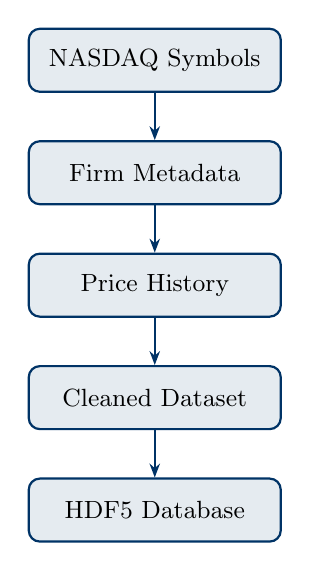
\begin{tikzpicture}[
  node distance=0.6cm,
  box/.style={draw=darkblue, thick, rounded corners, fill=darkblue!10, 
              minimum width=3.2cm, minimum height=0.8cm, align=center,
              font=\small},
  arr/.style={-{Stealth[length=5pt]}, thick, darkblue}
]
\node[box] (sym) {NASDAQ Symbols};
\node[box, below=of sym] (meta) {Firm Metadata};
\node[box, below=of meta] (prices) {Price History};
\node[box, below=of prices] (clean) {Cleaned Dataset};
\node[box, below=of clean] (hdf) {HDF5 Database};

\draw[arr] (sym) -- (meta);
\draw[arr] (meta) -- (prices);
\draw[arr] (prices) -- (clean);
\draw[arr] (clean) -- (hdf);
\end{tikzpicture}
\end{columns}

\end{frame}
%
%..................................................................
%
\begin{frame}{What the Dataset Contains}

\begin{columns}[T]
\column{0.48\textwidth}
\begin{block}{\textbf{[M]}\ \ Equity Metadata}
\begin{itemize}
  \item Company name, sector, industry
  \item Market capitalisation
  \item Descriptive attributes from Yahoo Finance
  \item One record per ticker
\end{itemize}
\end{block}

\column{0.48\textwidth}
\begin{block}{\textbf{[P]}\ \ Adjusted Price Series}
\begin{itemize}
  \item Open, High, Low, Close, Volume
  \item Adjusted for splits and dividends
  \item Multi-index: \texttt{(ticker, date)}
  \item Long historical horizon
\end{itemize}
\end{block}
\end{columns}

\vspace{0.6cm}

\begin{block}{\textbf{[D]}\ \ Storage Format --- HDF5}
Hierarchical Data Format allows fast I/O for large numerical arrays. \\
Keys: \texttt{stocks/info} (metadata) and \texttt{stocks/prices/adjusted} (prices).
\end{block}

\end{frame}
%
%..................................................................
%
\begin{frame}{What is HDF5?}

\textbf{HDF5} (Hierarchical Data Format v5) is an open-source binary file format
designed for storing and organizing \textbf{large, complex datasets}.

\medskip

\begin{columns}[T]
\begin{column}{0.52\textwidth}
\textbf{Core concepts}
\begin{itemize}
  \item \textbf{Groups} --- folder-like containers that form a tree hierarchy (like a filesystem inside a file)
  \item \textbf{Datasets} --- typed, multidimensional arrays of any size
  \item \textbf{Attributes} --- lightweight key--value metadata attached to groups or datasets
\end{itemize}
\end{column}

\begin{column}{0.44\textwidth}
\centering
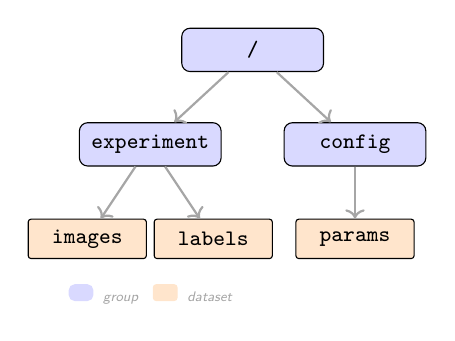
\begin{tikzpicture}[
  grp/.style={draw, rounded corners=3pt, fill=blue!15,
              minimum width=1.8cm, minimum height=0.55cm,
              font=\footnotesize\ttfamily, align=center},
  ds/.style={draw, rounded corners=1pt, fill=orange!20,
             minimum width=1.5cm, minimum height=0.5cm,
             font=\footnotesize\ttfamily, align=center},
  arr/.style={->, thick, gray!70},
  lbl/.style={font=\tiny\sffamily\itshape, text=gray!70},
]
% Root
\node[grp] (root) at (0, 0) {/};

% Level 1
\node[grp] (exp)  at (-1.3, -1.2) {experiment};
\node[grp] (conf) at ( 1.3, -1.2) {config};

% Level 2
\node[ds] (img) at (-2.1, -2.4) {images};
\node[ds] (lab) at (-0.5, -2.4) {labels};
\node[ds] (par) at ( 1.3, -2.4) {params};

% Edges
\draw[arr] (root) -- (exp);
\draw[arr] (root) -- (conf);
\draw[arr] (exp)  -- (img);
\draw[arr] (exp)  -- (lab);
\draw[arr] (conf) -- (par);

% Legend
\node[lbl] at (-1.3, -3.1) {%
  \tikz\fill[blue!15,draw,rounded corners=2pt] (0,0) rectangle (0.3,0.2);
  ~group\quad
  \tikz\fill[orange!20,draw,rounded corners=1pt] (0,0) rectangle (0.3,0.2);
  ~dataset};
\end{tikzpicture}
\end{column}
\end{columns}

\end{frame}
%
%..................................................................
%
\begin{frame}[fragile]{Why Use HDF5?}

\begin{columns}[T]
\begin{column}{0.54\textwidth}
\textbf{Key advantages}
\begin{enumerate}
  \item \textbf{Scalability} --- handles datasets from kilobytes to terabytes in a single file
  \item \textbf{Fast I/O} --- supports chunked storage and built-in compression (gzip, lz4, \ldots); enables partial reads without loading the whole file
  \item \textbf{Self-describing} --- metadata travels with the data, improving reproducibility
  \item \textbf{Portable} --- platform-independent binary format; one file works on Linux, macOS, Windows
  \item \textbf{Broad ecosystem} --- native support in Python (\texttt{h5py}, \texttt{pandas}), MATLAB, R, C/C++, Julia, \ldots
\end{enumerate}
\end{column}

\begin{column}{0.42\textwidth}
\textbf{HDF5 vs.\ alternatives}
\small
\smallskip
\centering
\renewcommand{\arraystretch}{1.15}
\begin{tabular}{@{}lccc@{}}
\toprule
\textbf{Feature} & \textbf{HDF5} & \textbf{CSV} & \textbf{NPY} \\
\midrule
N-dim arrays     & \checkmark & ---        & \checkmark \\
Compression      & \checkmark & ---        & ---        \\
Partial read     & \checkmark & ---        & ---        \\
Metadata         & \checkmark & ---        & ---        \\
Multi-dataset    & \checkmark & ---        & ---        \\
Human-readable   & ---        & \checkmark & ---        \\
\bottomrule
\end{tabular}

\end{column}
\end{columns}

\end{frame}
%
%..................................................................
%
\begin{frame}{End-to-End Pipeline}

\centering
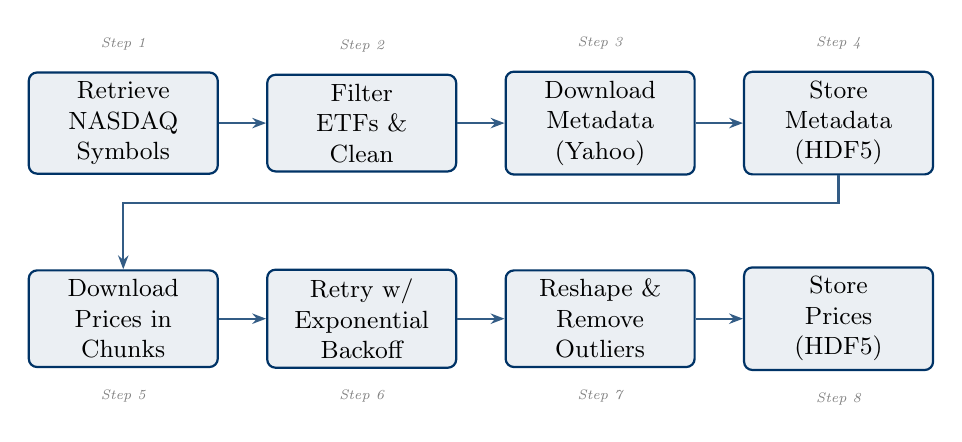
\begin{tikzpicture}[
  node distance=0.55cm and 0.6cm,
  stage/.style={draw=darkblue, thick, rounded corners=3pt, fill=darkblue!8,
                minimum width=2.4cm, minimum height=1.1cm, align=center, font=\small},
  arr/.style={-{Stealth[length=5pt]}, thick, darkblue!80},
  lbl/.style={font=\tiny\itshape, text=gray}
]
% Row 1
\node[stage] (s1) {Retrieve\\NASDAQ\\Symbols};
\node[stage, right=of s1] (s2) {Filter\\ETFs \&\\Clean};
\node[stage, right=of s2] (s3) {Download\\Metadata\\(Yahoo)};
\node[stage, right=of s3] (s4) {Store\\Metadata\\(HDF5)};

% Row 2
\node[stage, below=1.2cm of s1] (s5) {Download\\Prices in\\Chunks};
\node[stage, right=of s5] (s6) {Retry w/\\Exponential\\Backoff};
\node[stage, right=of s6] (s7) {Reshape \&\\Remove\\Outliers};
\node[stage, right=of s7] (s8) {Store\\Prices\\(HDF5)};

\draw[arr] (s1) -- (s2);
\draw[arr] (s2) -- (s3);
\draw[arr] (s3) -- (s4);
\draw[arr] (s4.south) -- ++(0,-0.35) -| (s5.north);
\draw[arr] (s5) -- (s6);
\draw[arr] (s6) -- (s7);
\draw[arr] (s7) -- (s8);

\node[lbl, above=0.15cm of s1] {Step 1};
\node[lbl, above=0.15cm of s2] {Step 2};
\node[lbl, above=0.15cm of s3] {Step 3};
\node[lbl, above=0.15cm of s4] {Step 4};
\node[lbl, below=0.15cm of s5] {Step 5};
\node[lbl, below=0.15cm of s6] {Step 6};
\node[lbl, below=0.15cm of s7] {Step 7};
\node[lbl, below=0.15cm of s8] {Step 8};
\end{tikzpicture}

\end{frame}
%
%..................................................................
%
\begin{frame}[fragile]{Retrieving NASDAQ Symbols}

The notebook uses \texttt{pandas\_datareader} to obtain the full NASDAQ symbol directory.

\begin{lstlisting}
from pandas_datareader.nasdaq_trader import get_nasdaq_symbols

traded_symbols = get_nasdaq_symbols()
\end{lstlisting}

\vspace{0.3cm}

\begin{block}{Filtering Logic}
\begin{enumerate}
  \item \textbf{Exclude ETFs}: retain only individual equities (\texttt{\textasciitilde traded\_symbols.ETF})
  \item \textbf{Drop missing values}: remove NaN tickers
  \item \textbf{Cast to string \& strip}: ensure ticker format consistency
  \item \textbf{Deduplicate}: call \texttt{.unique()} to avoid repeated symbols
\end{enumerate}
\end{block}

Result: a clean Python list \texttt{all\_symbols} containing thousands of equity tickers.

\end{frame}
%
%..................................................................
%
\begin{frame}[fragile]{Downloading Firm-Level Metadata}

For each ticker, the notebook queries Yahoo Finance via \texttt{yfinance}:
\vspace{-.3cm}
\begin{tcolorbox}[
  colback=gray!5,
  colframe=gray!60,
  arc=4mm
]
\begin{lstlisting}
yf_symbols = yf.Tickers(all_symbols)
for ticker, yf_object in tqdm(yf_symbols.tickers.items()):
    info = yf_object.get_info()       # dict of attributes
    meta_data.append(pd.Series(info).to_frame(ticker))
\end{lstlisting}
\end{tcolorbox}
\vspace{-.5cm}
\begin{columns}[T]
\column{0.48\textwidth}
\begin{block}{Robustness Features}
\small
\begin{itemize}
  \item \textbf{try/except}: failures are logged, not fatal
  \item \textbf{Logging to file}: \texttt{yfinance\_download\_errors.log}
  \item \textbf{stderr redirect}: suppresses noisy library output
  \item \textbf{Progress bar}: via \texttt{tqdm}
\end{itemize}
\end{block}

\column{0.48\textwidth}
\begin{block}{Output}
\begin{itemize}
  \item A wide DataFrame: one row per ticker, many attribute columns
  \item Numeric conversion applied automatically
  \item Stored in HDF5 under key \texttt{stocks/info}
\end{itemize}
\end{block}
\end{columns}

\end{frame}
%
%..................................................................
%
\begin{frame}[fragile]{Downloading Prices --- Chunking \& Retry Strategy}
\footnotesize
\begin{lstlisting}
MAX_RETRIES  = 5
BASE_BACKOFF = 1.5
MIN_INTERVAL = 1.0
for i, chunk in enumerate(chunks(all_symbols, 100), 1):
    for attempt in range(1, MAX_RETRIES + 1):
        try:
            df = yf.download(chunk, period='max',
                             auto_adjust=True, threads=True)
            prices_adj.append(df.stack(-1))
            break
        except Exception as e:
            tm.sleep(BASE_BACKOFF ** attempt)  # exponential backoff
\end{lstlisting}

\normalsize
\begin{block}{Three Resilience Mechanisms}
\begin{description}
  \item[Chunking] Tickers are split into batches of 100 to avoid oversized API calls.
  \item[Retry + Backoff] Each failed chunk is retried up to 5 times; wait grows as $1.5^{\text{attempt}}$.
  \item[Rate Pacing] A 1-second pause between batches reduces rate-limit risk.
\end{description}
\end{block}

\end{frame}
%
%..................................................................
%
\begin{frame}[fragile]{Reshaping the Price DataFrame}

After downloading, the raw data is restructured:

\begin{lstlisting}
prices_adj = (pd.concat(prices_adj)
              .dropna(how='all', axis=1)
              .rename(columns=str.lower)
              .swaplevel())
prices_adj.index.names = ['ticker', 'date']
\end{lstlisting}
\small
\begin{columns}[T]
\column{0.48\textwidth}
\begin{block}{Index Structure}
A \textbf{MultiIndex} \texttt{(ticker, date)} enables:
\begin{itemize}
  \item Cross-sectional slicing (all stocks on one date)
  \item Time-series slicing (one stock over time)
  \item Efficient group-by operations
\end{itemize}
\end{block}

\column{0.48\textwidth}
\begin{block}{Columns (lowercase)}
\begin{itemize}
  \item \texttt{open}, \texttt{high}, \texttt{low}, \texttt{close}
  \item \texttt{volume}
  \item All prices are \textbf{split- and dividend-adjusted}
\end{itemize}
\end{block}
\end{columns}

\end{frame}
%
%..................................................................
%
\begin{frame}[fragile]{Outlier Removal}

Extreme return observations are likely data errors. The notebook uses a simple but effective filter:

\begin{lstlisting}
df = prices_adj.close.unstack('ticker')
pmax = df.pct_change().max()
pmin = df.pct_change().min()
to_drop = pmax[pmax > 1].index.union(pmin[pmin < -1].index)
prices_adj = prices_adj.drop(to_drop, level='ticker')
\end{lstlisting}

\vspace{0.3cm}

\begin{block}{Filtering Rule}
\begin{itemize}
  \item Compute daily returns: $r_t = (P_t - P_{t-1})/P_{t-1}$
  \item If \textbf{any} daily return exceeds $+100\%$ or falls below $-100\%$, the \textbf{entire ticker} is removed
  \item This guards against price errors that could distort empirical results
\end{itemize}
\end{block}

\end{frame}
%
%..................................................................
%
\begin{frame}[fragile]{Final Storage}

The cleaned dataset is written to HDF5 with a date filter:

\begin{lstlisting}
prices_adj.sort_index() \
    .loc[idx[:, '1990':'2019'], :] \
    .to_hdf(results_path / 'data_ip_2026.h5',
            'stocks/prices/adjusted')
\end{lstlisting}

\vspace{0.3cm}

\begin{block}{HDF5 Database Layout}
\centering
\begin{tabular}{lll}
\toprule
\textbf{Key} & \textbf{Content} & \textbf{Shape} \\
\midrule
\texttt{stocks/info} & Firm metadata & tickers $\times$ attributes \\
\texttt{stocks/prices/adjusted} & Adj.\ prices 1990--2019 & (ticker, date) $\times$ OHLCV \\
\bottomrule
\end{tabular}
\end{block}

\vspace{0.3cm}

This consolidated file can be loaded efficiently by downstream research notebooks.

\end{frame}
%__________________________________________________________________________
%
%\subsection{Summary of Part 2}
%__________________________________________________________________________
%
\begin{frame}{Summary of Part 2 \& Downstream Uses}

\begin{block}{What the Notebook Produces}
A single HDF5 file containing \textbf{firm metadata} and \textbf{adjusted prices} for thousands of U.S.\ equities spanning roughly three decades.
\end{block}

\vspace{0.3cm}

\begin{block}{Possible Applications}
\begin{itemize}
  \item \textbf{Factor modeling}: Fama--French, momentum, quality factors
  \item \textbf{Portfolio construction}: mean--variance, risk parity, Black--Litterman
  \item \textbf{Machine learning}: return prediction, regime detection, NLP on firm metadata
  \item \textbf{Market microstructure}: liquidity analysis, volatility estimation
\end{itemize}
\end{block}

\end{frame}
%__________________________________________________________________________
%
\section{Data Preparation and Feature Engineering}
%__________________________________________________________________________
%
\begin{frame}{Context: Conditional Autoencoders for Asset Pricing}

\begin{columns}[T]
\column{0.55\textwidth}
\begin{block}{The Bigger Picture}
Conditional autoencoders learn \textbf{latent factor structures} from asset returns,
where factor loadings depend on observable firm characteristics.

\medskip

This notebook is \textbf{Part~1} of the project:
it builds the \textbf{input dataset} that the neural network will consume.
\end{block}

\vspace{0.3cm}

\begin{alertblock}{Why Data Preparation Matters}
Model performance critically depends on \textbf{clean returns} and
\textbf{well-constructed features} --- ``garbage in, garbage out.''
\end{alertblock}

\column{0.4\textwidth}
\centering
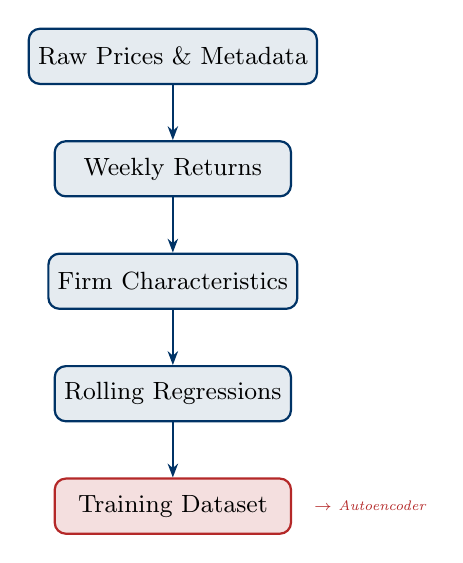
\begin{tikzpicture}[
  node distance=0.7cm,
  box/.style={draw=darkblue, thick, rounded corners, fill=darkblue!10,
              minimum width=3.0cm, minimum height=0.7cm, align=center,
              font=\small},
  arr/.style={-{Stealth[length=5pt]}, thick, darkblue}
]
\node[box] (d1) {Raw Prices \& Metadata};
\node[box, below=of d1] (d2) {Weekly Returns};
\node[box, below=of d2] (d3) {Firm Characteristics};
\node[box, below=of d3] (d4) {Rolling Regressions};
\node[box, below=of d4, fill=accent!15, draw=accent] (d5) {Training Dataset};

\draw[arr] (d1) -- (d2);
\draw[arr] (d2) -- (d3);
\draw[arr] (d3) -- (d4);
\draw[arr] (d4) -- (d5);

\node[font=\tiny\itshape, right=0.15cm of d5, text=accent] {$\rightarrow$ Autoencoder};
\end{tikzpicture}
\end{columns}

\end{frame}
%
%..................................................................
%
\begin{frame}{Notebook Workflow at a Glance}

\centering
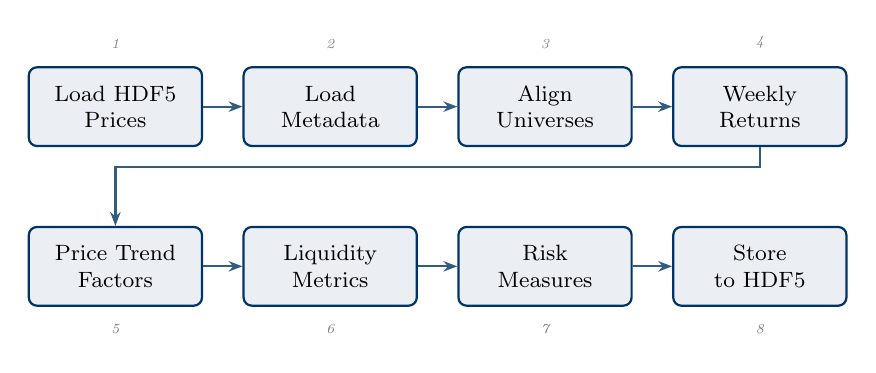
\begin{tikzpicture}[
  node distance=0.4cm and 0.5cm,
  stage/.style={draw=darkblue, thick, rounded corners=3pt, fill=darkblue!8,
                minimum width=2.2cm, minimum height=1.0cm, align=center, font=\footnotesize},
  arr/.style={-{Stealth[length=5pt]}, thick, darkblue!80},
  lbl/.style={font=\tiny\itshape, text=gray}
]
\node[stage] (s1) {Load HDF5\\Prices};
\node[stage, right=of s1] (s2) {Load\\Metadata};
\node[stage, right=of s2] (s3) {Align\\Universes};
\node[stage, right=of s3] (s4) {Weekly\\Returns};

\node[stage, below=1.0cm of s1] (s5) {Price Trend\\Factors};
\node[stage, right=of s5] (s6) {Liquidity\\Metrics};
\node[stage, right=of s6] (s7) {Risk\\Measures};
\node[stage, right=of s7] (s8) {Store\\to HDF5};

\draw[arr] (s1) -- (s2);
\draw[arr] (s2) -- (s3);
\draw[arr] (s3) -- (s4);
\draw[arr] (s4.south) -- ++(0,-0.25) -| (s5.north);
\draw[arr] (s5) -- (s6);
\draw[arr] (s6) -- (s7);
\draw[arr] (s7) -- (s8);

\node[lbl, above=0.1cm of s1] {1};
\node[lbl, above=0.1cm of s2] {2};
\node[lbl, above=0.1cm of s3] {3};
\node[lbl, above=0.1cm of s4] {4};
\node[lbl, below=0.1cm of s5] {5};
\node[lbl, below=0.1cm of s6] {6};
\node[lbl, below=0.1cm of s7] {7};
\node[lbl, below=0.1cm of s8] {8};
\end{tikzpicture}

\vspace{0.4cm}

\begin{columns}[T]
\column{0.32\textwidth}
\centering\small\textbf{Data Loading}\\[2pt]
\footnotesize Prices, metadata, universe alignment

\column{0.32\textwidth}
\centering\small\textbf{Feature Engineering}\\[2pt]
\footnotesize 14 firm-level characteristics

\column{0.32\textwidth}
\centering\small\textbf{Storage}\\[2pt]
\footnotesize HDF5 with hierarchical keys
\end{columns}

\end{frame}
%__________________________________________________________________________
%
\subsection{Data Loading \& Alignment}
%__________________________________________________________________________
%
\begin{frame}[fragile]{Loading Prices \& Metadata from HDF5}

\begin{lstlisting}
prices   = pd.read_hdf(results_path / 'data_ip_2026.h5',
                        'stocks/prices/adjusted')
metadata = pd.read_hdf(results_path / 'data_ip_2026.h5',
                        'stocks/info').rename(columns=str.lower)
\end{lstlisting}

\vspace{0.3cm}

\begin{columns}[T]
\column{0.48\textwidth}
\begin{block}{Prices}
\begin{itemize}
  \item MultiIndex: \texttt{(ticker, date)}
  \item Columns: \texttt{open, high, low, close, volume}
  \item Split- and dividend-adjusted
\end{itemize}
\end{block}

\column{0.48\textwidth}
\begin{block}{Metadata}
\begin{itemize}
  \item Index: \texttt{ticker}
  \item Key columns retained: \texttt{sector}, \texttt{marketcap}, \texttt{sharesoutstanding}
  \item Sourced from Yahoo Finance
\end{itemize}
\end{block}
\end{columns}

\end{frame}
%
%..................................................................
%
\begin{frame}[fragile]{Filtering \& Aligning the Ticker Universe}

Only tickers that pass \textbf{all} quality filters are retained:
\footnotesize
\begin{lstlisting}
tickers_with_metadata = metadata[
    metadata.sector.isin(sectors) &       # well-populated sectors (>50 firms)
    metadata.marketcap.notnull() &        # non-missing market cap
    metadata.sharesoutstanding.notnull() & # non-missing shares
    (metadata.sharesoutstanding > 0)       # positive shares
].index
valid_tickers = tickers_with_metadata.intersection(
    prices.index.get_level_values(0).unique())
prices = prices.loc[idx[valid_tickers, :], :]
\end{lstlisting}
\small
\vspace{-.3cm}
\begin{block}{Alignment Logic}
\begin{enumerate}
  \item Filter metadata: sector $> 50$ firms, valid \texttt{marketcap} and \texttt{sharesoutstanding}
  \item Intersect with tickers actually present in the price data
  \item Keep only the \textbf{common universe} in both datasets
\end{enumerate}
This guarantees every observation has both prices \emph{and} fundamentals.
\end{block}

\end{frame}
%__________________________________________________________________________
%
%\subsection{Weekly Returns}
%__________________________________________________________________________
%
\begin{frame}[fragile]{Constructing Weekly Returns}

\begin{lstlisting}
returns = (prices.close
           .unstack('ticker')        # wide format: dates x tickers
           .resample('W-FRI').last() # last price each Friday
           .sort_index()
           .pct_change()             # week-over-week returns
           .iloc[1:])               # drop first NaN row
\end{lstlisting}

\vspace{0.3cm}

\begin{columns}[T]
\column{0.48\textwidth}
\begin{block}{Why Weekly?}
\begin{itemize}
  \item Reduces daily microstructure noise
  \item Lowers dimensionality vs.\ daily data
  \item Better balance between resolution and statistical robustness
\end{itemize}
\end{block}

\column{0.48\textwidth}
\begin{block}{Design Choices}
\begin{itemize}
  \item \textbf{Friday-to-Friday} alignment ensures consistency
  \item \textbf{Adjusted prices} $\Rightarrow$ returns reflect total shareholder performance
  \item Result stored in HDF5 under \texttt{returns}
\end{itemize}
\end{block}
\end{columns}

\end{frame}
%__________________________________________________________________________
%
\subsection{Factor Engineering}
%__________________________________________________________________________
%
\begin{frame}{Overview of Engineered Features}

The notebook constructs \textbf{14 firm-level characteristics} organised into three categories:

\vspace{0.2cm}

\centering
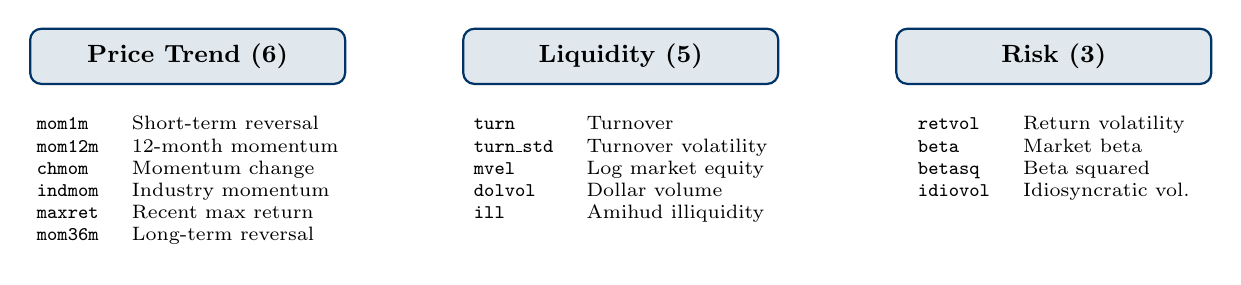
\begin{tikzpicture}[
  cat/.style={draw=darkblue, thick, rounded corners, fill=darkblue!12,
              minimum width=4.0cm, minimum height=0.7cm, align=center, font=\small\bfseries},
  item/.style={font=\scriptsize, align=left},
  node distance=0.3cm
]
% Category boxes
\node[cat] (c1) at (0,0) {Price Trend (6)};
\node[cat] (c2) at (5.5,0) {Liquidity (5)};
\node[cat] (c3) at (11,0) {Risk (3)};

% Items
\node[item, below=0.25cm of c1] (i1) {%
\begin{tabular}{@{}ll@{}}
\texttt{mom1m}  & Short-term reversal \\
\texttt{mom12m} & 12-month momentum \\
\texttt{chmom}  & Momentum change \\
\texttt{indmom} & Industry momentum \\
\texttt{maxret} & Recent max return \\
\texttt{mom36m} & Long-term reversal
\end{tabular}};

\node[item, below=0.25cm of c2] (i2) {%
\begin{tabular}{@{}ll@{}}
\texttt{turn}     & Turnover \\
\texttt{turn\_std} & Turnover volatility \\
\texttt{mvel}     & Log market equity \\
\texttt{dolvol}   & Dollar volume \\
\texttt{ill}      & Amihud illiquidity
\end{tabular}};

\node[item, below=0.25cm of c3] (i3) {%
\begin{tabular}{@{}ll@{}}
\texttt{retvol}  & Return volatility \\
\texttt{beta}    & Market beta \\
\texttt{betasq}  & Beta squared \\
\texttt{idiovol} & Idiosyncratic vol.
\end{tabular}};
\end{tikzpicture}

\vspace{0.3cm}

All factors are computed at \textbf{weekly (Friday)} frequency, aligned with the return panel, and stored in long format \texttt{(date, ticker)} in HDF5.

\end{frame}
%
%..................................................................
%
\begin{frame}{Price Trend Factors --- Definitions}
\small
Let $P_{i,t}$ be the adjusted closing price of stock $i$ at trading day $t$, and $M \approx 21$ trading days $\approx 1$ month.

\vspace{0.2cm}

\renewcommand{\arraystretch}{1.5}
\begin{tabular}{@{}lll@{}}
\toprule
\textbf{Factor} & \textbf{Formula} & \textbf{Interpretation} \\
\midrule
\texttt{mom1m} &
$\displaystyle\frac{P_{i,t}}{P_{i,t-M}} - 1$ &
Short-term reversal (1-month return)\\[4pt]
\texttt{mom12m} &
$\displaystyle\frac{P_{i,t-M}}{P_{i,t-12M}} - 1$ &
Momentum: 11-month return, skip last month \\[4pt]
\texttt{chmom} &
$\displaystyle R_{t-6:t-1} - R_{t-12:t-7}$ &
Momentum acceleration / deceleration \\[4pt]
\texttt{indmom} &
$\displaystyle\frac{1}{N_{s,t}}\sum_{i\in s} r^{(12m)}_{i,t}$ &
Equal-weighted sector 12-month return \\[4pt]
\texttt{maxret} &
$\displaystyle\max_{k} \frac{P_{i,k}}{P_{i,k-M}}-1$ &
Max 21-day return in prior month \\[4pt]
\texttt{mom36m} &
$\displaystyle\frac{P_{i,t-12M}}{P_{i,t-36M}} - 1$ &
Long-term reversal (months $t{-}36$ to $t{-}13$) \\
\bottomrule
\end{tabular}

\end{frame}
%
%..................................................................
%
\begin{frame}[fragile]{Price Trend --- Code Pattern}

All price-trend factors follow the same \texttt{pandas} chain:

\begin{lstlisting}
# Example: 12-month momentum (skip last month)
mom12m = (close
          .pct_change(periods=11 * MONTH)   # cumulative return
          .shift(MONTH)                      # skip most recent month
          .resample('W-FRI').last()          # align to Friday
          .stack()                           # long format
          .to_frame('mom12m'))               # named DataFrame
\end{lstlisting}

\vspace{0.2cm}

\begin{block}{Motivation}
\begin{itemize}
  \item \textbf{Skipping the last month} avoids contamination from short-term reversal
  \item Isolates \textbf{medium-term momentum}: past winners tend to keep winning
  \item \texttt{chmom} refines this by detecting whether momentum is \textbf{accelerating or decelerating}
\end{itemize}
\end{block}

\end{frame}
%
%..................................................................
%
\begin{frame}[fragile]{Industry Momentum --- Sector-Level Aggregation}

\texttt{indmom} is a \textbf{sector-level} control variable, broadcast to each stock:

\begin{lstlisting}
# Step 1: compute equal-weighted sector average 12-month return
indmom = (close.pct_change(12*MONTH).resample('W-FRI').last()
          .stack().to_frame('close')
          .join(metadata[['sector']])
          .groupby(['date','sector']).close.mean()
          .to_frame('indmom').reset_index())

# Step 2: broadcast sector value to every stock
indmom = (returns.stack().to_frame('ret')
          .join(metadata[['sector']]).reset_index()
          .merge(indmom)
          .set_index(['date','ticker']).loc[:, ['indmom']])
\end{lstlisting}

\vspace{0.2cm}

This separates \textbf{stock-specific momentum} from \textbf{industry-wide trends},
a standard control in cross-sectional asset pricing studies.

\end{frame}
%
%..................................................................
%
\begin{frame}[fragile]{Liquidity Metrics}

\renewcommand{\arraystretch}{1.4}
\begin{tabular}{@{}lp{9cm}@{}}
\toprule
\textbf{Factor} & \textbf{Definition} \\
\midrule
\texttt{turn} & 3-month average daily volume $\div$ shares outstanding \\
\texttt{turn\_std} & Std.\ dev.\ of daily share turnover over 1 month \\
\texttt{mvel} & $\ln\!\bigl(1 + \text{price-scaled market cap}\bigr)$ \\
\texttt{dolvol} & $\ln\!\bigl(1 + \text{avg.\ daily dollar volume, lagged 1 month}\bigr)$ \\
\texttt{ill} & Amihud illiquidity: $\displaystyle\frac{1}{M}\sum_{k}\frac{|r_{i,k}|}{V_{i,k}\cdot P_{i,k}}$ \\
\bottomrule
\end{tabular}

\vspace{0.4cm}

\begin{columns}[T]
\column{0.48\textwidth}
\begin{block}{Amihud (2002) Measure}
Captures \textbf{price impact}: illiquid stocks move more per unit of traded value.\\
Higher values $\Rightarrow$ less liquid.
\end{block}

\column{0.48\textwidth}
\begin{block}{Log Transforms}
Dollar volume and market equity use $\ln(1+x)$ to handle \textbf{right-skewed distributions} and stabilise variance.
\end{block}
\end{columns}

\end{frame}
%
%..................................................................
%
\begin{frame}[fragile]{Liquidity --- Sample Code}

\begin{lstlisting}
# Turnover: 3-month average volume / shares outstanding
turn = (volume.rolling(3*MONTH).mean()
        .resample('W-FRI').last()
        .div(metadata.sharesoutstanding)
        .stack('ticker').to_frame('turn'))

# Amihud illiquidity: mean( |daily return| / dollar volume )
dv  = close.mul(volume)
ill = (close.pct_change().abs().div(dv)
       .rolling(21).mean()
       .resample('W-FRI').last()
       .stack().to_frame('ill'))
\end{lstlisting}

\vspace{0.2cm}

All liquidity factors share the same pattern: compute a daily quantity, apply a rolling window, resample to weekly Fridays, and reshape to long format.

\end{frame}
%
%..................................................................
%
\begin{frame}[fragile]{Risk Measures --- Market Beta}

\textbf{Market proxy}: equal-weighted cross-sectional mean of weekly returns.

\begin{lstlisting}
index = (close.resample('W-FRI').last().pct_change()
         .mean(axis=1).to_frame('x'))
\end{lstlisting}

\vspace{0.15cm}

\textbf{Rolling OLS} over a 3-year (156-week) window:

\begin{lstlisting}
def get_market_beta(y, x=index):
    df = x.join(y.to_frame('y')).dropna()
    model = RollingOLS(endog=df.y,
                       exog=sm.add_constant(df[['x']]),
                       window=3*52)
    return model.fit(params_only=True).params['x']

beta = (returns.dropna(thresh=3*52, axis=1)
        .apply(get_market_beta).stack().to_frame('beta'))
\end{lstlisting}
\end{frame}
%
%..................................................................
%
\begin{frame}[fragile]{Risk Measures --- Market Beta}

The estimated beta at week $t$ is:
$$
\hat\beta_{i,t} = \frac{\sum_{k=t-155}^{t}(x_k - \bar x)(r_{i,k} - \bar r_i)}{\sum_{k=t-155}^{t}(x_k - \bar x)^2}
$$

\end{frame}
%
%..................................................................
%
\begin{frame}[fragile]{Risk Measures --- Volatility \& Idiosyncratic Risk}

\begin{block}{\texttt{retvol} --- Return Volatility}
Standard deviation of daily returns over the prior month:
\begin{lstlisting}
retvol = (close.pct_change()
  .rolling(21).std()
  .resample('W-FRI').last()
  .stack()
  .to_frame('retvol'))
\end{lstlisting}
\end{block}
\end{frame}
%
%..................................................................
%
\begin{frame}[fragile]{Risk Measures --- Volatility \& Idiosyncratic Risk}
\begin{block}{\texttt{idiovol} --- Idiosyncratic Volatility}
Residual std.\ dev.\ from a market-model regression over 3 years:
\begin{lstlisting}
def get_ols_residuals(y, x=index):
    df = x.join(y.to_frame('y')).dropna()
    model = sm.OLS(df.y,
      sm.add_constant(df[['x']]))
    return model.fit().resid.std()
\end{lstlisting}
Applied via \texttt{rolling(3*52).apply(...)}.
\end{block}
\end{frame}
%
%..................................................................
%
\begin{frame}[fragile]{Risk Measures --- Volatility \& Idiosyncratic Risk}

\begin{block}{\texttt{betasq} --- Beta Squared}
Simply $\hat\beta_{i,t}^2$. Captures \textbf{non-linear} exposure to market risk;
relevant because expected returns may depend on higher moments of factor loadings.
\end{block}

\end{frame}
%__________________________________________________________________________
%
\subsection{Storage \& Output}
%__________________________________________________________________________
%
\begin{frame}[fragile]{HDF5 Database Layout}

All outputs are stored in a single HDF5 file under hierarchical keys:

\begin{lstlisting}
with pd.HDFStore(results_path / 'autoencoder_reloaded.h5') as store:
    store.put('close', close)
    store.put('volume', volume)
    store.put('returns', returns)
    store.put('metadata', metadata)
\end{lstlisting}
\end{frame}
%
%..................................................................
%
\begin{frame}[fragile]{HDF5 Database Layout}

\centering
\small
\begin{tabular}{lll}
\toprule
\textbf{HDF5 Key} & \textbf{Content} & \textbf{Index} \\
\midrule
\texttt{close} / \texttt{volume} & Daily prices / volume (wide) & date $\times$ ticker \\
\texttt{returns} & Weekly returns (wide) & date $\times$ ticker \\
\texttt{metadata} & Sector, mktcap, shares & ticker \\
\midrule
\texttt{factor/mom1m} & Short-term reversal & (date, ticker) \\
\texttt{factor/mom12m} & Momentum & (date, ticker) \\
\texttt{factor/chmom} & Momentum change & (date, ticker) \\
\texttt{factor/indmom} & Industry momentum & (date, ticker) \\
\texttt{factor/maxret} & Recent max return & (date, ticker) \\
\texttt{factor/mom36m} & Long-term reversal & (date, ticker) \\
\texttt{factor/turn} \ldots\ \texttt{factor/ill} & Liquidity metrics & (date, ticker) \\
\texttt{factor/beta} \ldots\ \texttt{factor/idiovol} & Risk measures & (date, ticker) \\
\bottomrule
\end{tabular}

\end{frame}
%__________________________________________________________________________
%
\subsection{Summary of Part 3}
%__________________________________________________________________________
%
\begin{frame}{Summary \& Next Steps}

\begin{block}{What This Notebook Produces}
A structured HDF5 file containing \textbf{weekly returns} and \textbf{14 firm-level
characteristics} for thousands of U.S.\ equities, all aligned on a consistent
\texttt{(date, ticker)} panel at Friday frequency.
\end{block}

\vspace{-0.2cm}

\begin{columns}[T]
\column{0.48\textwidth}
\begin{block}{Key Design Principles}
\begin{itemize}
  \item Universe alignment: prices $\cap$ metadata
  \item Consistent weekly (Friday) sampling
  \item Rolling windows for time-varying features
  \item Economic motivation for every factor
\end{itemize}
\end{block}

\column{0.48\textwidth}
\begin{block}{Downstream Usage (Next Chapter)}
\begin{itemize}
  \item \textbf{Conditioning variables} for the autoencoder's encoder network
  \item \textbf{Cross-sectional normalisation} (rank transforms)
  \item \textbf{Train / validation / test} split
  \item \textbf{Latent factor extraction} and SDF estimation
\end{itemize}
\end{block}
\end{columns}
\end{frame}
%
%===================================================================================================
%
\end{document}